\section{Bias--variance tradeoff}
\subsection{Expectation means averaging over a specified source of variation}
\label{sec:reg:expect}
An expectation is a probability-weighted average, not necessarily the average of the particular observations in hand. For a discrete $Z$, $\E[Z]=\sum_z zp(z)$; with a density, $\E[Z]=\int z p(z)\,dz$. A conditional expectation uses a restricted population: $\E[Y\mid X=x]=\int y p(y\mid x)\,dy$ [S2]. For continuous $X$, this refers to a conditional distribution, rather than division by the probability of the zero-probability event $X=x$.

In the slide's seven-person table, the empirical height distribution assigns probabilities $2/7,4/7,1/7$ to $160,170,180$. Its mean is $1180/7\approx168.57$. Restricting to the three rows labelled $f$ changes the probabilities to $2/3,1/3,0$, and the conditional empirical mean becomes $490/3\approx163.33$. These are averages under the table's empirical distribution; population means need not equal them.

Linearity, $\E[aZ+bV]=a\E[Z]+b\E[V]$, follows by distributing a sum or integral and needs no independence. In contrast,
\[
\E[ZV]=\E[Z]\E[V]+\operatorname{Cov}(Z,V).
\]
Thus factorization holds for uncorrelated variables (with the necessary moments). Independence is sufficient but stronger. The universally valid conditional calculation is
\begin{equation}
\E[ZV]=\E_Z\!\left[Z\E[V\mid Z]\right].
\label{eq:reg:tower}
\end{equation}
At fixed $Z=z$, $z$ is a constant and can be pulled out; the outer expectation then averages over $Z$. This is the tower property applied to the product.

\begin{warning}[Clarification of slide S3]
The slide labels a factorization ``uncorrelated'' but its intermediate averaging notation can suggest that $\E[V\mid Z]=\E[V]$. Uncorrelatedness alone does not justify this intermediate substitution. The final factorization follows from zero covariance; independence (or mean independence in the required direction) justifies that substitution. We will explicitly condition whenever taking a factor outside an expectation.
\end{warning}
\paragraph{Optional counterexample.} Let $Z$ be uniform on $\{-1,0,1\}$ and $V=Z^2$. Symmetry gives $\E[ZV]=\E[Z^3]=0=\E[Z]\E[V]$, so they are uncorrelated. Yet $\E[V\mid Z]=Z^2$ varies with $Z$, and $V$ is completely determined by $Z$.

\subsection{Three functions, two experiments}
\label{sec:reg:random}
The notation in S4--S8 distinguishes three essential objects:
\begin{center}\small
\begin{tabular}{p{.19\linewidth}p{.39\linewidth}p{.31\linewidth}}
\toprule Symbol & Meaning & What is averaged?\\\midrule
$\bar y(x)$ & True conditional mean $\E[Y\mid X=x]$ & Fresh labels at the same input\\
$\hat f(x;\mathcal D)$ & Prediction after fitting one dataset & Nothing: one fitted predictor\\
$\bar f(x)$ & Mean fitted prediction $\E_{\mathcal D}[\hat f(x;\mathcal D)]$ & Repeated training datasets\\\bottomrule
\end{tabular}
\end{center}
The bar in $\bar y$ and $\bar f$ therefore represents different averaging operations. In the sine mechanism $\bar y(x)=\sin(2\pi x)$; it is not the observed noisy label. The function $\bar f$ is a theoretical average over repetitions, not generally a model we obtain from our one observed training set.

\paragraph{Experiment 1: freeze one trained model.} Once $\mathcal D$ is observed and fitting is deterministic, its learned weights are fixed. Draw a new independent pair $(X,Y)\sim\mathcal P$. Its loss is random because the pair is random. The risk of that fitted predictor is
\begin{equation}
R(\mathcal D)=\E_{X,Y}[(\hat f(X;\mathcal D)-Y)^2\mid\mathcal D]
=\iint(\hat f(x;\mathcal D)-y)^2p(x,y)\,dy\,dx.
\label{eq:reg:risk}
\end{equation}
Why the double integral? At every possible pair $(x,y)$ we calculate its squared loss, weight it by how likely that pair is, and sum continuously over both coordinates. It is the expectation definition applied to the \emph{function} $L(X,Y)$, not an expectation that updates the weights. Integrating over $y$ first averages possible labels at an input; integrating over $x$ averages how often each input appears.

\paragraph{Experiment 2: repeat the entire learning process.} Before collecting data, $\mathcal D\sim\mathcal P^N$ is random: each repetition provides $N$ fresh i.i.d. examples. A fixed degree and fixed fitting rule map each dataset to coefficients, so $\hat\theta(\mathcal D)$ and $\hat f(x;\mathcal D)$ become random across repetitions, even at a fixed query $x$. Now evaluate the \emph{procedure} by
\begin{equation}
\mathcal R=\E_{\mathcal D}[R(\mathcal D)]
=\iiint(\hat f(x;\mathcal D)-y)^2p(x,y)p(\mathcal D)\,d\mathcal D\,dy\,dx.
\end{equation}
The product density expresses independence of fresh test data and training data. For i.i.d. training samples, $p(\mathcal D)=\prod_{i=1}^N p(x_i,y_i)$; $d\mathcal D$ stands for integration over every training coordinate and label (or sums for discrete parts). We do not need to compute this enormous integral explicitly to reason about it. If the algorithm is randomized, include its random seed in the outer expectation too.

\paragraph{Why training MSE is only a proxy [S5].} For a predictor fixed independently of a sample, the sample mean of its losses estimates its population risk; with integrability, a law of large numbers explains convergence. But the fitted predictor is chosen using the training sample. Its training losses have been optimized, so this argument does not automatically establish that its training MSE is an unbiased estimate of its risk. A fresh test set restores independence for evaluation conditional on the fitted model. This is precisely the gap that overfitting exploits.

\paragraph{Reconstruction prompt (A3).} At a fixed $x$, list which of $Y$, $\bar y(x)$, $\hat f(x;\mathcal D)$, and $\bar f(x)$ vary when (i) only a new label is drawn, and (ii) only the training dataset is redrawn. Why is a single fitted model's error not itself its bias?

\subsection{Derive the decomposition at one input first}
\label{sec:reg:proof}
\paragraph{Assumptions.} We use squared loss and finite second moments, including $\E_{\mathcal D}[\hat f(x;\mathcal D)^2]<\infty$ at the inputs considered. A fresh test pair is independent of training data. Fix the training-set size and the learning rule. Let
\[
m=\bar y(x),\quad a=\bar f(x),\quad F=\hat f(x;\mathcal D),\quad
\sigma^2(x)=\Var(Y\mid X=x).
\]
For this derivation $x,m,a$ are fixed; $F$ varies over training sets and $Y$ varies over fresh conditional labels. This separation prevents most notation mistakes.

\paragraph{Step 1: separate variation between fitted models [S9--S10].}
Add and subtract the mean fitted prediction $a$:
\[
F-Y=(F-a)+(a-Y).
\]
Squaring and using linearity gives
\begin{align}
\E_{\mathcal D,Y\mid x}[(F-Y)^2]
&=\E_{\mathcal D}[(F-a)^2]+\E_{Y\mid x}[(a-Y)^2]\notag\\
&\quad+2\E_{Y\mid x}\!\left[(a-Y)\E_{\mathcal D}[F-a]\right].
\label{eq:reg:first}
\end{align}
For the cross term we first fix $x,y$, so $(a-y)$ is constant with respect to the dataset average. Test--training independence means this dataset average is the ordinary training-set average, unaffected by that fresh label. By the definition of $a$,
\[
\E_{\mathcal D}[F-a]=\E_{\mathcal D}[F]-a=a-a=0.
\]
Thus the cross term vanishes. Its \emph{individual realizations need not vanish}: positive and negative deviations cancel when averaged. The first remaining term is prediction variance $\Var_{\mathcal D}(F)$.

\paragraph{Pause (A4).} Explain why this reasoning can fail if $Y$ is one of the labels used to fit $F$. Identify the specific averaging step that changes; do not merely say ``overfitting.''

\paragraph{Step 2: separate mean-model error from unpredictable labels [S11].}
There is still variation inside $a-Y$. Insert the true conditional mean:
\[
a-Y=(a-m)+(m-Y).
\]
Now $a-m$ is constant under the label average, so
\begin{align}
\E_{Y\mid x}[(a-Y)^2]
&=(a-m)^2+\E_{Y\mid x}[(m-Y)^2]
 +2(a-m)\E_{Y\mid x}[m-Y]\notag\\
&=(a-m)^2+\sigma^2(x),
\end{align}
because $\E[Y\mid x]=m$. Notice that this second cancellation needs a zero \emph{conditional} mean, not merely $\E[m(X)-Y]=0$ globally.

\begin{keyidea}[Pointwise decomposition]
Define $b(x)=\bar f(x)-\bar y(x)$ and $v(x)=\E_{\mathcal D}[(\hat f(x;\mathcal D)-\bar f(x))^2]$. Then
\begin{equation}
\boxed{\E_{\mathcal D,Y\mid x}[(\hat f(x;\mathcal D)-Y)^2]
=b(x)^2+v(x)+\sigma^2(x).}
\label{eq:reg:decomp}
\end{equation}
Bias $b(x)$ is signed; the additive error contribution is \emph{bias squared}. All three terms on the right are nonnegative and have squared target units.
\end{keyidea}
Gaussian noise is unnecessary for this identity. Nor must noise variance be constant in $x$. Finite moments and the stated sampling conditions are what matter.

\paragraph{Step 3: average across inputs [S12].}
Use $p(x,y)=p(y\mid x)p(x)$ and the tower property:
\begin{equation}
\mathcal R=\E_X[b(X)^2]+\E_X[v(X)]+\E_X[\sigma^2(X)].
\label{eq:reg:integrated}
\end{equation}
The first term is the \emph{mean squared pointwise bias}, not $(\E_X[b(X)])^2$: opposite signed biases at different inputs must not cancel a prediction penalty. The lecture's extra $y$ subscript on the bias-squared expectation is harmless but unnecessary because its integrand no longer depends on $y$.

\paragraph{Why the conditional mean is the right target.}
For any fixed scalar prediction $c$ at $x$, the same second expansion yields
\[
\E[(c-Y)^2\mid x]=(c-\bar y(x))^2+\sigma^2(x).
\]
The second term cannot be changed by $c$; the first is minimized at $c=\bar y(x)$. Thus conditional-mean prediction is optimal under squared loss. ``Noise'' is irreducible \emph{given the available input information and distribution}; a new informative sensor feature may reduce it. It is not necessarily metaphysical randomness or measurement error alone.

\subsection{Interpret the components without confusing their experiments}
\label{sec:reg:interpret}
\textbf{Bias squared:} How far is the average predictor from the conditional mean? A consistently wrong shape across datasets suggests bias. \textbf{Variance:} How far do individual fitted predictions scatter around their own average at the same input? It is not variation of predictions across different inputs and not simply variance of the labels. \textbf{Noise:} How much do fresh labels vary around their conditional mean even if that mean were known?

\paragraph{Worked numerical example.} At one input the mean target is $2$, fresh-label variance is $0.25$, and three equally likely training outcomes predict $1,2,3$. Their average is $2$, so $b^2=0$ and $v=(1+0+1)/3=2/3$. Expected fresh-label squared error is $2/3+1/4=11/12$. For a direct check, let fresh labels be $1.5$ and $2.5$ with equal probabilities, independent of the model outcome. For predictions $1,2,3$, average squared losses are respectively $1.25,0.25,1.25$; averaging these gives $11/12$ again. Each fitted model may be imperfect even though the learning procedure has zero bias here.

\paragraph{Partially worked example (A5).} Shift the three predictions to $2,3,4$, retaining the same label distribution. Their mean is now $3$, hence $b=3-2=1$. Complete the variance and total-error calculations. Does translating all predictions change their spread?

\paragraph{Reading the lecture's pictures [S7, S13--S14].} In S7, each thin line is a model trained on a different dataset, while the highlighted mean line averages their predictions at each fixed $x$. A flat mean near zero can be stable yet miss the sine shape. In the darts analogy [S13], the bullseye corresponds to the true target, each dart to a retrained prediction, the dart cloud's centre to $\bar f$, and its spread to prediction variance. For scalar regression the darts would lie on a line; the two-dimensional board is only an analogy. It does not depict label noise unless an additional source of target variation is shown.

In S14, columns (a) and (b) show fixed functions repeated across $\mathcal D_1,\mathcal D_2,\mathcal D_3$: at a given input their dataset-induced variance is zero, even though their bias may be large and differs across inputs. Column (c) learns a cubic; column (d) learns an affine function. Both can vary across datasets. The illustration suggests flexibility versus stability, but three drawings cannot quantify population bias or variance, and do not prove a universal ordering.

\paragraph{Answering the lecture's consistent-error question.} A procedure that makes the same \emph{systematic prediction error relative to the conditional mean} across many training sets suggests high bias. The qualification matters: fresh noisy labels can cause unavoidable errors even for an unbiased predictor, and a single dataset cannot identify the components. Bias concerns a learning procedure and a target, not just the visible residual of one fitted model.

\subsection{A computational experiment that separates the sources}
\label{sec:reg:experiment}
\paragraph{Prediction and task (A6).} Before reading the reference code in the solutions: fit degrees $0,3,9$ to repeated noisy sine datasets. Predict which degree has the highest bias and which has the highest prediction variance. At a fixed input grid, store predictions in a matrix $P\in\R^{B\times G}$, where $B$ is the number of retrainings and $G$ the number of query inputs. Decide which axis to average. Explain why one model evaluated at many inputs is not a substitute for retraining.

The companion experiment fixes 12 training locations and redraws independent Gaussian label noise with $\sigma=0.15$ for 400 repetitions. This is a \emph{fixed-design variant} of the lecture's random-design experiment: the outer average is over noisy labels conditional on the chosen training inputs. It isolates one source of instability; it does not estimate the additional effect of random input locations. Evaluation averages over a uniform grid of 201 inputs, approximating a uniform input distribution. Degree 9 uses least squares, not interpolation of all 12 points.

At each grid point compute the replicate mean $\hat a$, mean squared deviation from $\hat a$, and squared deviation of $\hat a$ from the known sine mean. With divisor $B$ (not $B-1$), the finite-array identity
\[
\frac1B\sum_{r=1}^B(P_{rg}-m_g)^2
=(\hat a_g-m_g)^2+\frac1B\sum_{r=1}^B(P_{rg}-\hat a_g)^2
\]
is exact up to floating-point error. This verifies the algebra; the components are still Monte Carlo estimates of population quantities. Add the known $0.15^2$ noise variance to obtain conditional expected fresh-label MSE. A separate draw of independent test noise gives a noisy empirical check rather than an exact equality.
\begin{figure}[htbp]\centering
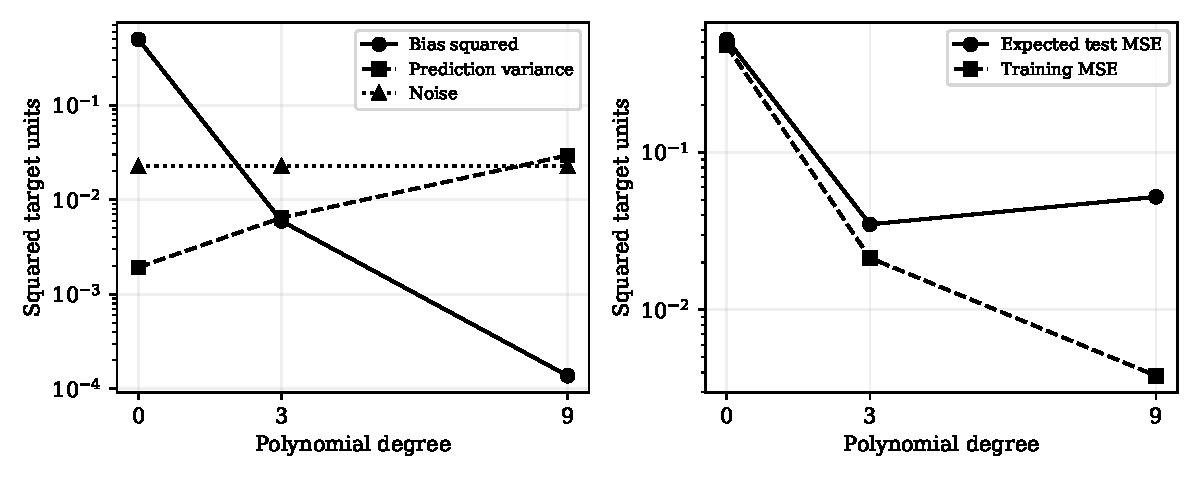
\includegraphics[width=.94\linewidth]{bias_variance/components.pdf}
\caption{Executed fixed-design experiment. Left: estimated integrated bias squared, prediction variance, and noise. Right: their sum compared with average training MSE. Logarithmic vertical scales separate the magnitudes; lines only connect the tested degrees. A lower training error need not mean a lower expected test error.}
\end{figure}
\begin{center}\small
\begin{tabular}{rrrrrr}
\toprule Degree & Training MSE & Bias$^2$ & Variance & Expected test & Noisy test\\
\midrule
0 & 0.47609 & 0.49753 & 0.00193 & 0.52195 & 0.52203\\
3 & 0.02136 & 0.00595 & 0.00645 & 0.03490 & 0.03489\\
9 & 0.00381 & 0.00014 & 0.02946 & 0.05209 & 0.05202\\
\bottomrule
\end{tabular}
\end{center}

The middle degree balances approximation and instability in this constructed setting. No rule says every test-error curve must be U-shaped. The exact decomposition survives cases where that familiar cartoon does not describe the behavior. Regularization will next provide another way to control the fitted procedure's sensitivity, beyond choosing the degree.

\subsection*{Compact reference sheet}
\begin{center}\small
\begin{tabular}{p{.40\linewidth}p{.49\linewidth}}
\toprule Quantity / equation & Meaning, conditions, use\\\midrule
$\hat R=N^{-1}\|\Phi\theta-\mathbf y\|^2$ & Observed training objective; $\Phi$ is $N\times(M+1)$. Fit coefficients, not certify generalization.\\
$R(\mathcal D)=\E_{X,Y}[(\hat f-Y)^2\mid\mathcal D]$ & Risk of one frozen fitted predictor on independent fresh data.\\
$\bar y(x)=\E[Y\mid x]$ & Squared-loss optimal target; requires a finite conditional second moment for this risk argument.\\
$\bar f(x)=\E_{\mathcal D}[\hat f(x;\mathcal D)]$ & Average over a specified retraining experiment, with fixed learning rule and sample size.\\
$b(x)=\bar f(x)-\bar y(x)$ & Signed systematic error of that procedure at one input.\\
$v(x)=\Var_{\mathcal D}(\hat f(x;\mathcal D))$ & Prediction sensitivity across training datasets at fixed $x$.\\
$\sigma^2(x)=\Var(Y\mid x)$ & Residual uncertainty given the input; can vary with $x$.\\
$\mathcal R=\E_X[b^2+v+\sigma^2]$ & Squared-loss decomposition; independent test data and finite moments.\\\bottomrule
\end{tabular}
\end{center}
